% Design 
%!TEX root = ../Project.tex
\section{Design}

\subsection{Methodologies}
\label{sub:methodologies}
The Model, View, Controller (MVC) design paradigm was chosen to be used to structure the project. The MVC design patten has many benefits as discussed below.  

%TODO

\subsection{Engine}
The main considerations  for the engine was to it made it configureable as possible. To achieve this everything was designed in term of interfaces, which allowed the particular implementation to be changed. The objects themselves were loaded from their serialised form on disk. 

\subsubsection{Data Format}
XMl was chosen as the data format for this project. The main reason is that it is human readable, this allow me to create and test the data format before the editor was created.

XML schema is a way of validating a  xml document. A schema was produced for each serialised object\footnote{in the \texttt{schemas} directory}. 
The main benefit of this was to testing of hand written xml I used before the editor was created. It also helped ensure that the xml produced by the editor was correct.  

The data was design to be extendable, as well as provide implementations of the various assets the advance user can specify their own custom classes. As an example there four weapons types provided by the engine,

\begin{lstlisting}[language=xml, caption=]

\end{lstlisting}


\subsubsection{Assets}
All the assets used in the model including weapons, maps and even the units themselves are configured via the xml data format.  


\subsection{Game Progression}
\begin{figure}[htbp]
	\centering
		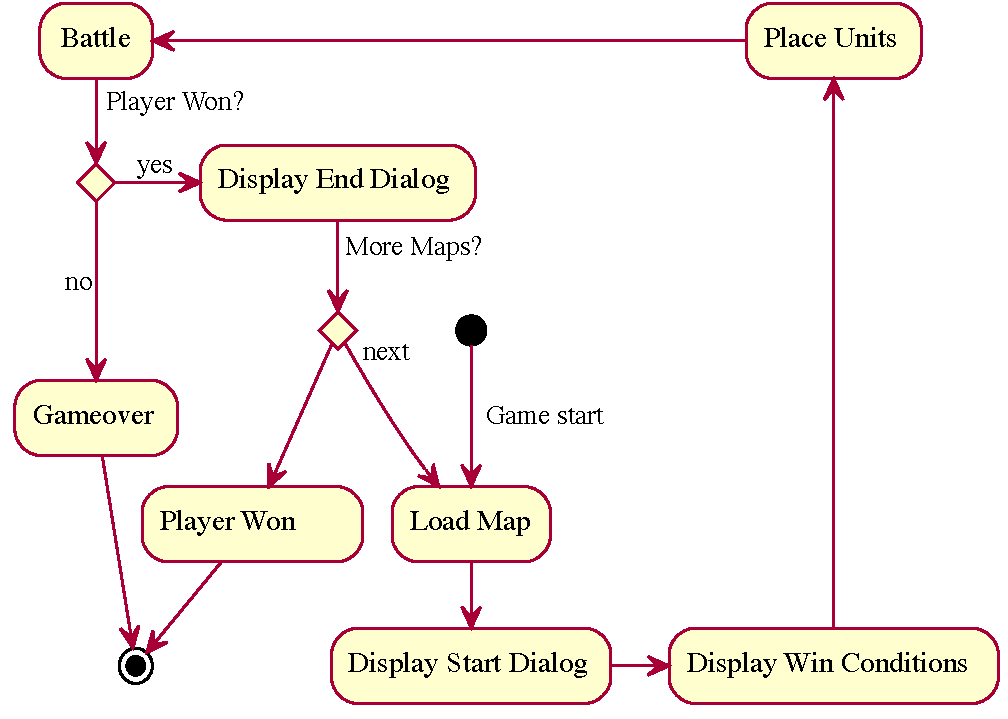
\includegraphics[height=3in]{figures/game.pdf}
	\caption{Activity diagram which a high level of overview of the engine}
	\label{fig:figures_game}
\end{figure}

Figure \ref{fig:figures_game} shows the overview of how the created game progress.  Each game has a number of maps where a battle take place. After the map is loaded any relanent dialog is display, along with winning conditions. The player's units are then placed are the map\footnote{While the engine support allowing the user's to choose where the their units are placed, the GUI does not due to time constraints. The editor does support specify the starting location for the player's units}.  And the battle (which will be discussed below takes). If the player's loses the battle, a gameover screen is shown and the game end. In contrast if the player wins he/she advances to the next map, if there one.    

\subsection{Gui}

The 

\begin{figure}[hb]
	\centering
		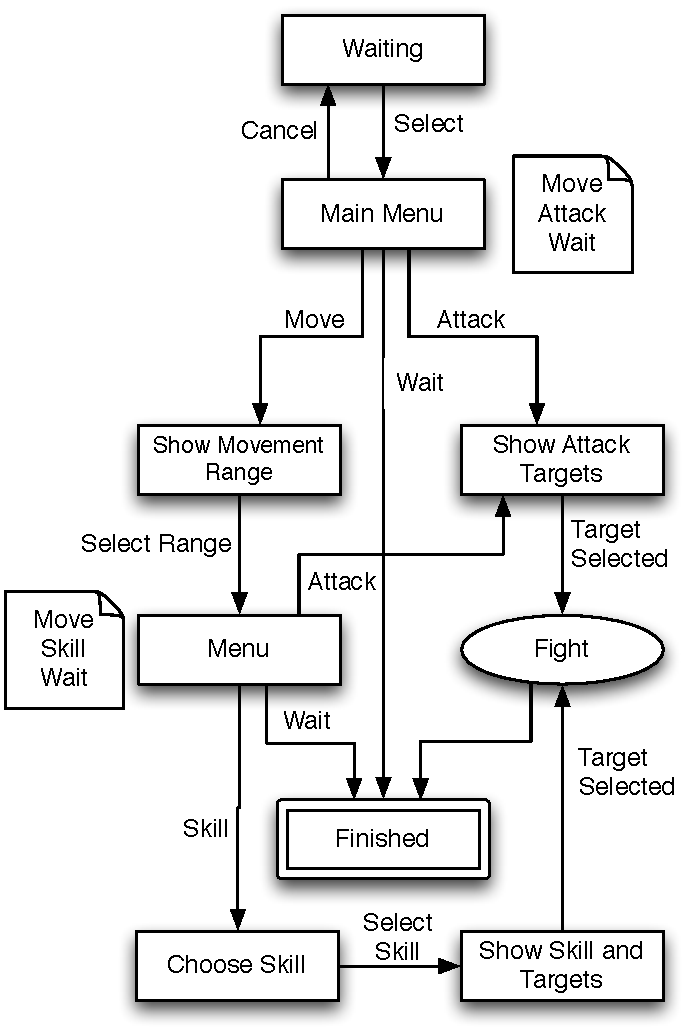
\includegraphics[width=4in]{figures/unit.pdf}
	\caption{The State diagram of a single turn of a player's unit}
	\label{fig:figures_unit}
\end{figure}

\subsection{View}

\subsubsection{Tilemap}
\label{sub:tilemap}


There were two main choices for the isometric tilemap, a `Diamond' map or a  `Staggered' map \cite{isometric_game_programming}, examples of both are shown below.

\def\tilemapSize{5in}
\begin{figure}[htbp]
	\begin{center}

	\subfigure[Diamond Map]{
		\label{fig:tilemap1} 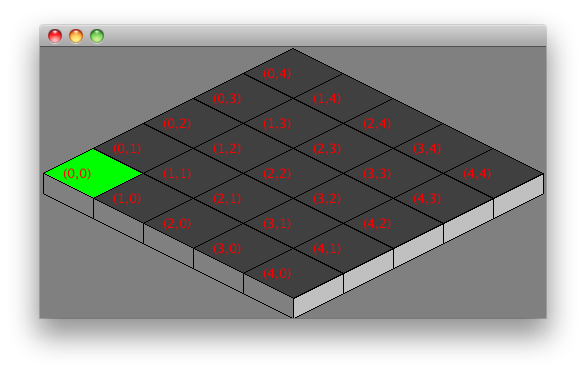
\includegraphics[width=\tilemapSize]{figures/tilemap1.png}} 
	\subfigure[Staggered Map]{
		\label{fig:tilemap2} 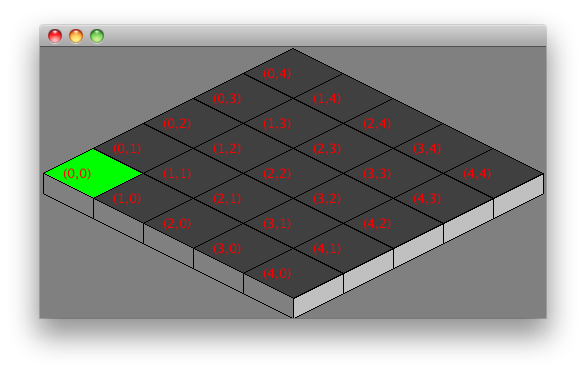
\includegraphics[width=\tilemapSize]{figures/tilemap2.png}} 
	\caption{\label{fig:tilemap0} The two main types of isometric tilemaps}
	\end{center}
\end{figure}

The `Staggered' Map has following advantages:
\begin{itemize}
	\item The map fill up the screen with very little wasted space, so the user can more of what happing on the map.
\end{itemize} 

The `Diamond' map was chosen for the following reasons:
\begin{itemize}
	\item `Diamond' map look nicer then `Staggered' maps because it has no ragged edges.
	\item Since that maps are large (at lest 15 \* 15) the space wasted at the edges of the map does not matter as much.
	% TODO Check deegres (45?)
	\item Simpler to think about, since a `Diamond' map is just a rectangular map rotated.
\end{itemize}

\underline{Maths about isometric tilemaps? }



\subsection{Editor}

\subsubsection{Exporting}
%TODO put in implementation?
The editor can export a project as a complete package, either as a Mac OS X application or as jar. These application don't requires any external resources, apart from a recent version of java \footnote{specifically Java 1.6+}.

A notable feature of the editor is that jar will work on any java enabled platform, since the jar contains all required libraries for each platform. The OS X application can even be export on other platforms.

While most of the testing was done on OS X \footnote{Mac OS X 10.6 Snow leopard}, it also works well on Linux \footnote{Science  Linux x.y}. It even has limited compatibly with Windows\footnote{Tested on Windows 7 32 bit} (apart from some minor graphics issues).